% Systems Overview
% MIT License
%
% Copyright (c) 2026 HumberASV
% Copyright (c) 2026 Carson Fujita
%
% Permission is hereby granted, free of charge, to any person obtaining a copy
% of this software and associated documentation files (the "Software"), to deal
% in the Software without restriction, including without limitation the rights
% to use, copy, modify, merge, publish, distribute, sublicense, and/or sell
% copies of the Software, and to permit persons to whom the Software is
% furnished to do so, subject to the following conditions:
%
% The above copyright notice and this permission notice shall be included in all
% copies or substantial portions of the Software.
%
% THE SOFTWARE IS PROVIDED "AS IS", WITHOUT WARRANTY OF ANY KIND, EXPRESS OR
% IMPLIED, INCLUDING BUT NOT LIMITED TO THE WARRANTIES OF MERCHANTABILITY,
% FITNESS FOR A PARTICULAR PURPOSE AND NONINFRINGEMENT. IN NO EVENT SHALL THE
% AUTHORS OR COPYRIGHT HOLDERS BE LIABLE FOR ANY CLAIM, DAMAGES OR OTHER
% LIABILITY, WHETHER IN AN ACTION OF CONTRACT, TORT OR OTHERWISE, ARISING FROM,
% OUT OF OR IN CONNECTION WITH THE SOFTWARE OR THE USE OR OTHER DEALINGS IN THE
% SOFTWARE.
\section{Systems Overview}
The Loon-E \hyperref[itm:asv]{ASV} is an autonomous surface vehicle designed to operate on water. It is not equipped to be underwater; please don't try to submerge it. 
Loon-E is designed to be modular and adaptable, allowing for various configurations and payloads to suit different tasks as competition requirements evolve \autocite{HUMBERASVREPORT2026}.

\begin{figure}[h]
    \centering
    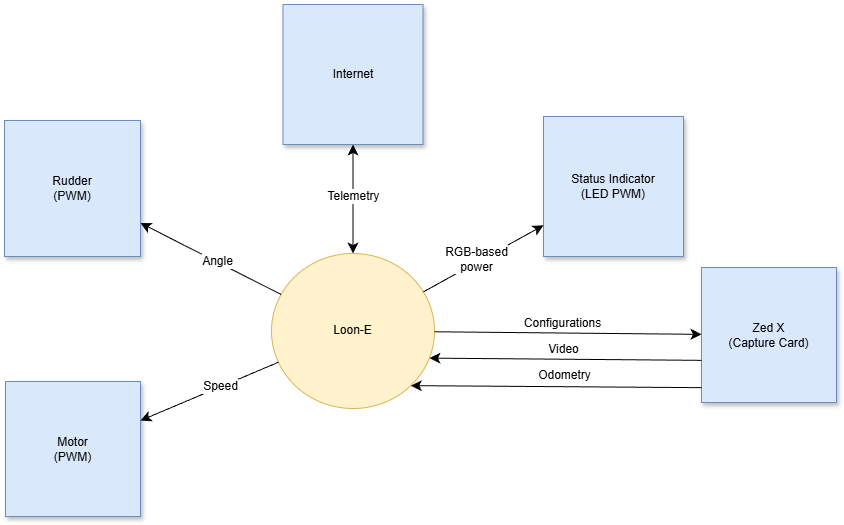
\includegraphics[width=0.8\textwidth]{./images/system_context.png}
    \caption{System Context Diagram}
    \label{fig:context-diagram}
\end{figure}

%TODO: Talk to electrical team about the electrical system and add a section on it here.

